% Chapitre 2 : Combinaison de classifieurs
\chapter{Combinaison de classifieurs}

\section*{Introduction}

L'évolution de l'apprentissage automatique a franchi une étape décisive avec l'émergence des
systèmes de classifieurs multiples (\emph{Multiple Classifier Systems -- MCS}), plus communément
désignés sous le terme d'apprentissage d'ensemble~\cite{luisfredgs_mcs_intro,wikip_ensemble_learning,heutte_combi_classif}. Cette approche repose sur un paradigme
fondamental : la combinaison stratégique de plusieurs modèles de prédiction pour pallier les
insuffisances inhérentes à tout classifieur unique.

Historiquement, la recherche en intelligence artificielle s'est concentrée sur l'optimisation
d'algorithmes individuels. Cependant, l'expérience a démontré qu'un modèle unique, aussi sophistiqué soit-il, est souvent limité par ses propres biais structurels et sa sensibilité au bruit des
données. L'apprentissage d'ensemble propose de substituer au modèle solitaire un comité de
décideurs dont la sagesse collective surpasse les capacités individuelles.

Cette section propose une exploration de la combinaison de classifieurs, structurée autour des
fondements théoriques, des typologies méthodologiques et des considérations architecturales
qui définissent ce domaine. L'analyse s'attache à montrer comment la diversité des modèles et la
rigueur de leur agrégation permettent d'atteindre des niveaux de performance et de robustesse
inaccessibles aux approches classiques.

\section{Définition et phases de la combinaison de classifieurs}

La \textbf{combinaison de classifieurs} est définie comme le processus d'intégration des sorties de
plusieurs modèles d'apprentissage afin de générer une décision globale plus fiable et précise.
Un système multi-classifieurs est structurellement composé d'un ensemble d'apprenants de
base, souvent qualifiés d'\emph{apprenants faibles} (\emph{weak learners}) lorsqu'ils sont pris isolément,
et d'un mécanisme de fusion qui orchestre leurs réponses.

Le cycle de vie d'un tel système se décompose généralement en trois phases critiques :

\begin{enumerate}
  \item \textbf{Génération de l'ensemble} : cette phase initiale consiste à produire un pool de modèles
  de base. L'objectif est de créer des modèles qui ne sont pas seulement performants,
  mais surtout complémentaires. La complémentarité est assurée par l'introduction de
  diversité, que ce soit par l'utilisation de différents sous-ensembles de données, de
  paramètres variés pour un même algorithme, ou de familles d'algorithmes distinctes.

  \item \textbf{Sélection ou élagage (\emph{pruning})} : une fois le pool généré, il peut être nécessaire de
  réduire la taille de l'ensemble. L'élagage vise à éliminer les modèles redondants ou ceux
  dont la performance dégrade la décision collective. Cette étape permet non seulement
  d'améliorer la précision globale mais aussi de réduire les coûts computationnels lors de
  l'inférence.

  \item \textbf{Combinaison ou fusion} : la phase finale consiste à fusionner les prédictions des
  modèles sélectionnés pour obtenir la réponse ultime. Le choix de la fonction de
  combinaison dépend crucialement du type d'information fournie par les classifieurs de
  base (niveau d'information en sortie).
\end{enumerate}

\subsection{Nature des sorties et niveaux d'information}

L'efficacité de la combinaison dépend de la richesse des informations transmises par les
modèles individuels. On distingue classiquement trois niveaux de sortie :

\begin{itemize}
  \item \textbf{Niveau \og Classe \fg{} (hard output)} : le classifieur fournit uniquement l'étiquette de la
  classe prédite. C'est l'information la plus élémentaire, où chaque modèle agit comme un
  votant binaire.

  \item \textbf{Niveau \og Rang \fg{}} : le classifieur produit une liste ordonnée des classes possibles, de la
  plus probable à la moins probable. Ce format est particulièrement utile lorsque la classe
  réelle ne figure pas au premier rang mais reste parmi les premières propositions.

  \item \textbf{Niveau \og Mesure \fg{} (soft output)} : c'est le niveau le plus riche. Le classifieur associe à
  chaque classe une valeur numérique, telle qu'une probabilité ou un score de confiance.
  Cette mesure quantifie l'incertitude du modèle et permet des fusions pondérées beaucoup
  plus fines.
\end{itemize}

Le tableau suivant présente une comparaison structurelle de ces types d'informations en sortie.

\begin{table}[h]
  \centering
  \caption{Comparaison des niveaux d'information en sortie des classifieurs}
    \small
    \begin{tabularx}{\textwidth}{lXlX}
    \toprule
    Type de sortie & Information contenue & Complexité de fusion & Cas d'utilisation typique \\
    \midrule
    Classe   & Étiquette discrète uniquement      & Faible  & Vote majoritaire simple \\
    Rang     & Préférences relatives ordonnées    & Moyenne & Méthode de Borda, systèmes de recommandation \\
    Mesure   & Probabilités, scores de confiance  & Élevée  & Moyenne pondérée, stacking, modèles bayésiens \\
    \bottomrule
  \end{tabularx}
\end{table}

\section{Motivations théoriques et justifications statistiques}

La supériorité des systèmes multi-classifieurs n'est pas une simple observation empirique ; elle
s'appuie sur des piliers théoriques robustes, notamment le théorème du jury de Condorcet et
la décomposition biais--variance~\cite{turing_ensemble_learning,analyticsvidhya_ensemble_learning,gfg_ensemble_learning}.

\subsection{Théorème du jury de Condorcet}

Formulé à l'origine dans le contexte des sciences sociales, ce théorème constitue une base
théorique fondamentale pour l'apprentissage d'ensemble~\cite{wikip_jury_theorem,cmu_ensembles_pdf}. Il postule que si un groupe
d'individus doit prendre une décision binaire (par exemple, classer un objet comme $A$ ou $B$)
et que chaque individu a une probabilité $p$ supérieure à $0{,}5$ de choisir la bonne réponse,
alors la probabilité que la décision de la majorité soit correcte augmente avec le nombre
d'individus.

Mathématiquement, si $L$ est le nombre de classifieurs indépendants et $p$ leur précision
individuelle, la probabilité $P$ que l'ensemble prenne la bonne décision par vote majoritaire
tend vers $1$ lorsque $L$ tend vers l'infini. À l'inverse, si $p < 0{,}5$, l'ajout de classifieurs réduit
la performance globale. Cette démonstration justifie l'utilisation d'\og apprenants faibles \fg{}
pour construire des systèmes puissants, à condition qu'ils soient plus performants qu'un tirage
aléatoire et qu'ils soient suffisamment indépendants.

\subsection{Décomposition biais--variance}

D'un point de vue statistique, l'erreur de généralisation d'un modèle d'apprentissage peut être
décomposée en trois composantes : le biais au carré, la variance et l'erreur irréductible (bruit)~\cite{wikip_bias_variance,utd_ensemble_lecture}.
La formule de l'erreur quadratique moyenne (MSE) est :

\begin{equation}
  \mathbb{E}\bigl[(y - \hat{f}(x))^2\bigr]
  = \operatorname{Bias}\bigl[\hat{f}(x)\bigr]^2
  + \operatorname{Var}\bigl[\hat{f}(x)\bigr]
  + \sigma^2,
\end{equation}

où $\sigma^2$ représente le bruit inhérent aux données.

\begin{itemize}
  \item Le \textbf{biais} mesure l'écart entre la prédiction moyenne du modèle et la valeur réelle. Un biais
  élevé est le signe d'un modèle trop simpliste qui ne capture pas la complexité des
  données (sous-apprentissage, \emph{underfitting}).

  \item La \textbf{variance} mesure la dispersion des prédictions pour différents jeux de données
  d'apprentissage. Une variance élevée indique que le modèle est trop sensible aux
  fluctuations et au bruit des données (sur-apprentissage, \emph{overfitting}).
\end{itemize}

L'apprentissage d'ensemble permet de naviguer dans ce compromis biais--variance. Les
méthodes de type bagging agissent principalement en réduisant la variance par la moyenne de
modèles complexes, tandis que les méthodes de boosting se concentrent sur la réduction du
biais en agrégeant itérativement des modèles simples pour corriger leurs erreurs systématiques.

\subsection{Théorie unifiée de la diversité dans les ensembles}

Une contribution th{\'e}orique importante aux m{\'e}thodes d'ensemble consiste {\`a} faire appara{\^i}tre
explicitement la diversit{\'e} comme composante de la d{\'e}composition de la perte. Pour une vaste
famille de fonctions de perte (notamment les divergences de Bregman, qui incluent l'erreur
quadratique moyenne et l'entropie crois{\'e}e), on peut montrer que la perte de l'ensemble s'exprime
comme la moyenne des pertes individuelles diminu{\'e}e d'un terme de diversit{\'e}~\cite{kuncheva_diversity_ensemble}.

Dans le cas particulier de l'erreur quadratique moyenne, cette id{\'e}e est captur{\'e}e par
l'identit{\'e} de Krogh et Vedelsby~\cite{krogh_vedelsby_ambiguity}. Pour un ensemble de $M$ mod{\`e}les
dont les pr{\'e}dictions sont $q_1(x),\dots,q_M(x)$ pour une entr{\'e}e $x$ et une cible $y$, on pose
\[
  \bar{q}(x) = \frac{1}{M} \sum_{i=1}^M q_i(x).
\]
L'identit{\'e} s'\'ecrit alors :
\begin{equation}
  \bigl(\bar{q}(x) - y\bigr)^2
  = \frac{1}{M} \sum_{i=1}^M \bigl(q_i(x) - y\bigr)^2
    - \frac{1}{M} \sum_{i=1}^M \bigl(q_i(x) - \bar{q}(x)\bigr)^2.
\end{equation}

Le membre de gauche est l'erreur quadratique de l'ensemble, le premier terme {\`a} droite la moyenne
des erreurs quadratiques individuelles, et le second terme (souvent appel{\'e} \og ambigu{\"i}t{\'e} \fg{} ou
\og diversit{\'e} \fg{}) mesure le degr{\'e} de d{\'e}saccord entre les pr{\'e}dictions des mod{\`e}les.
L'identit{\'e} montre que, toutes choses {\'e}gales par ailleurs, l'erreur de l'ensemble diminue lorsque
la diversit{\'e} augmente.

\paragraph{D{\'e}monstration de l'identit{\'e} de Krogh et Vedelsby.}
Pour simplifier les notations, on note $\bar{q} = \bar{q}(x)$ et $q_i = q_i(x)$.

\emph{(i) D{\'e}veloppement de l'erreur de l'ensemble.}
\[
  (\bar{q} - y)^2 = \bar{q}^2 - 2 \bar{q} y + y^2.
\]

\emph{(ii) D{\'e}veloppement de la moyenne des erreurs individuelles.}
\begin{align}
  \frac{1}{M} \sum_{i=1}^M (q_i - y)^2
  &= \frac{1}{M} \sum_{i=1}^M (q_i^2 - 2 q_i y + y^2) \\
  &= \frac{1}{M} \sum_{i=1}^M q_i^2 - 2 y \left( \frac{1}{M} \sum_{i=1}^M q_i \right) + y^2 \\
  &= \frac{1}{M} \sum_{i=1}^M q_i^2 - 2 y \bar{q} + y^2.
\end{align}

\emph{(iii) D{\'e}veloppement du terme de diversit{\'e}.}
\begin{align}
  \frac{1}{M} \sum_{i=1}^M (q_i - \bar{q})^2
  &= \frac{1}{M} \sum_{i=1}^M (q_i^2 - 2 q_i \bar{q} + \bar{q}^2) \\
  &= \frac{1}{M} \sum_{i=1}^M q_i^2 - 2 \bar{q} \left( \frac{1}{M} \sum_{i=1}^M q_i \right) + \bar{q}^2 \\
  &= \frac{1}{M} \sum_{i=1}^M q_i^2 - 2 \bar{q}^2 + \bar{q}^2 \\
  &= \frac{1}{M} \sum_{i=1}^M q_i^2 - \bar{q}^2.
\end{align}

\emph{(iv) Soustraction des deux termes.}
\begin{align}
  \frac{1}{M} \sum_{i=1}^M (q_i - y)^2
  - \frac{1}{M} \sum_{i=1}^M (q_i - \bar{q})^2
  &= \left( \frac{1}{M} \sum_{i=1}^M q_i^2 - 2 y \bar{q} + y^2 \right)
   - \left( \frac{1}{M} \sum_{i=1}^M q_i^2 - \bar{q}^2 \right) \\
  &= - 2 y \bar{q} + y^2 + \bar{q}^2 \\
  &= (\bar{q} - y)^2.
\end{align}

On retrouve bien l'identit{\'e} annonc{\'e}e. Comme le terme de diversit{\'e} est une somme de carr{\'e}s,
il est toujours positif ou nul. L'erreur de l'ensemble est donc toujours inf{\'e}rieure ou {\'e}gale
{\`a} la moyenne des erreurs individuelles, avec {\'e}galit{\'e} lorsque tous les mod{\`e}les pr{\'e}disent la m{\^e}me
valeur (diversit{\'e} nulle).

Cette identit{\'e} justifie l'importance
de promouvoir la diversit{\'e} dans les ensembles (via le bagging, le boosting, la randomisation
des architectures, etc.) et ouvre sur des g{\'e}n{\'e}ralisations {\`a} d'autres pertes au moyen des divergences
de Bregman~\cite{kuncheva_diversity_ensemble}.

\subsection{Les problèmes de Dietterich}

Thomas Dietterich a identifié trois raisons fondamentales expliquant pourquoi un ensemble
peut surpasser un modèle unique :

\begin{enumerate}
  \item \textbf{Le problème statistique} : lorsque le volume de données est faible par rapport à la taille
  de l'espace des hypothèses, l'algorithme peut trouver plusieurs modèles qui s'ajustent
  parfaitement aux données d'entraînement. En les combinant, l'ensemble réduit le risque
  de choisir par erreur un modèle qui généralise mal.

  \item \textbf{Le problème computationnel} : de nombreux algorithmes (comme les réseaux de
  neurones) utilisent des heuristiques de recherche locale qui peuvent rester bloquées
  dans des optima locaux. Un ensemble effectuant plusieurs recherches à partir de points
  de départ différents a plus de chances de trouver une meilleure approximation globale.

  \item \textbf{Le problème de représentation} : parfois, la véritable fonction cible ne peut être
  représentée par aucun des modèles de l'espace d'hypothèses choisi. La combinaison de
  plusieurs modèles permet d'étendre cet espace et d'approcher des fonctions plus
  complexes.
\end{enumerate}

\section{Achirtectures des systèmes multi-classifieurs}

L'architecture d'un système multi-classifieurs définit la manière dont les informations circulent
entre les composants et la façon dont les ressources sont exploitées.

\subsection{Architectures de contrôle de flux}

On distingue trois organisations principales :

\begin{enumerate}
  \item \textbf{Architecture parallèle} : tous les classifieurs opèrent indépendamment et
  simultanément. La fusion intervient à la fin. Cette structure est neutre (aucun classifieur
  n'influence les autres) et hautement parallélisable sur du matériel multi-c\oe urs.

  \item \textbf{Architecture séquentielle (en série)} : les classifieurs sont organisés en cascade. Un
  premier classifieur rapide effectue une prédiction ; s'il échoue ou exprime une faible
  confiance, l'exemple est passé à un second modèle plus complexe. Cela permet
  d'économiser des ressources de calcul en ne sollicitant les modèles coûteux que pour les
  cas difficiles.

  \item \textbf{Architecture hybride} : elle combine les deux approches. Par exemple, un premier étage
  parallèle peut générer un consensus, dont le résultat est validé par un classifieur de
  contrôle séquentiel.
\end{enumerate}

Ces formes peuvent être illustrées par des figures dédiées aux architectures parallèle et
séquentielle.

\begin{figure}[h]
  \centering
  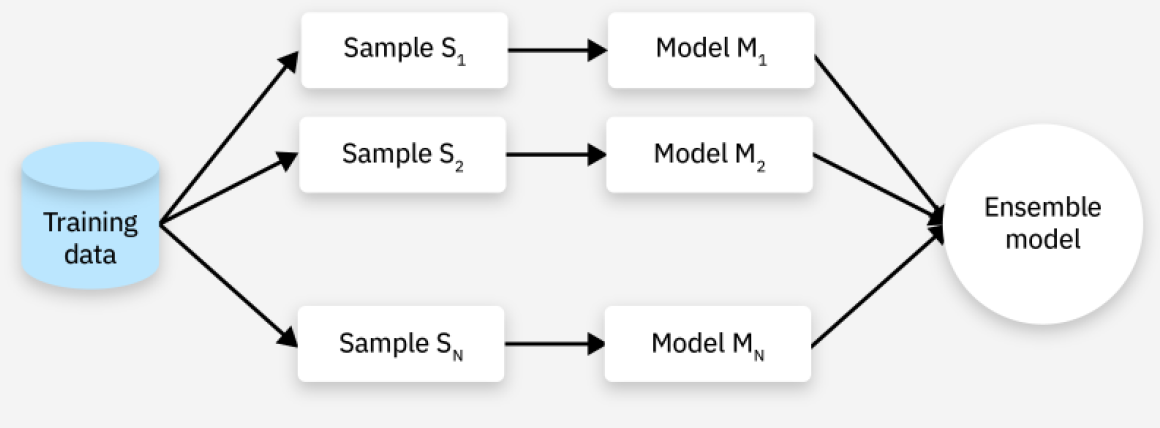
\includegraphics[width=0.9\textwidth]{chapitre1/figures/Architecture parallele.png}
  \caption{Architecture parallèle pour un système multi-classifieurs.}
  \label{fig:mcs-arch-parallel}
\end{figure}

\begin{figure}[h]
  \centering
  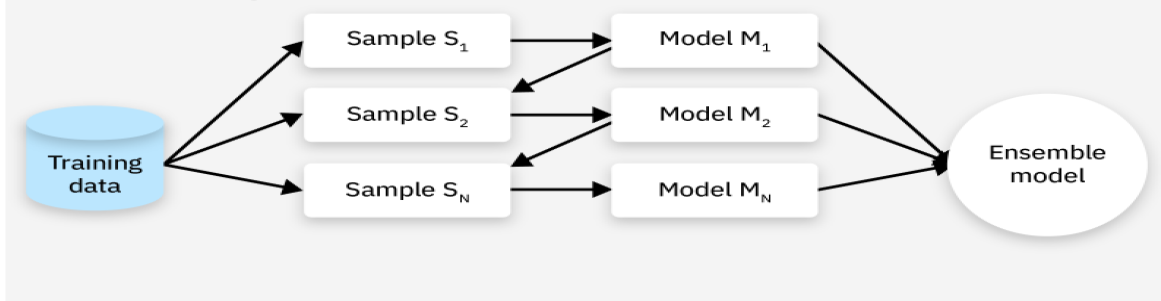
\includegraphics[width=0.9\textwidth]{chapitre1/figures/Architecture sequentielle.png}
  \caption{Architecture séquentielle pour un système multi-classifieurs.}
  \label{fig:mcs-arch-sequential}
\end{figure}

\subsection{Systèmes de sélection dynamique (DS)}

Une tendance majeure consiste à ne pas utiliser tous les classifieurs pour chaque exemple,
mais à sélectionner \og à la volée \fg{} le ou les modèles les plus compétents~\cite{cruz_deslib_jmlr,deslib_github,ko2007_dynamic_ensemble,esann2014_des_regression,deslib_docs}.

\begin{itemize}
  \item \textbf{Logique de compétence locale} : on définit une \og région de compétence \fg{} autour d'un
  exemple test (en utilisant par exemple ses plus proches voisins dans le jeu d'entraînement).
  On évalue ensuite quels modèles du pool ont été les plus performants dans cette zone
  spécifique.

  \item \textbf{DCS (dynamic classifier selection)} : on choisit l'unique meilleur modèle pour l'exemple
  donné.

  \item \textbf{DES (dynamic ensemble selection)} : on construit un sous-ensemble de modèles
  experts pour cette région particulière.
\end{itemize}



\section{Typologies des méthodes d'ensemble}

Les méthodes d'ensemble se divisent principalement en approches parallèles (bagging),
séquentielles (boosting) et hiérarchiques (stacking)~\cite{mlm_bagging_vs_boosting_vs_stacking,younas_bagging_boosting_stacking,nsacademy_what_is_ensemble}.

\subsection{Bagging (bootstrap aggregating)}

Le bagging (pour \emph{bootstrap aggregating}) vise à réduire la variance en entraînant plusieurs
modèles indépendants en parallèle sur des échantillons de données légèrement différents.
Introduit par Breiman~\cite{breiman_bagging_1996} et largement diffusé ensuite
~\cite{ibm_bagging,greatlearning_bagging_boosting,analyticsvidhya_ensemble_learning}, il est
particulièrement efficace pour des apprenants de base instables comme les arbres de décision
profonds.

\paragraph{Définition.}
À partir d'un ensemble d'apprentissage $D = \{(x_j, y_j)\}_{j=1}^n$, le bagging construit $m$
échantillons bootstrap $D_i$ par tirage aléatoire avec remise, chacun de taille $n$. Sur chaque
$D_i$, on entraîne un modèle de base $\hat{f}_i$ (\emph{base learner}). À la prédiction, les sorties
des $m$ modèles sont agrégées :
\begin{itemize}
  \item en régression, par moyenne
  \[
    \hat{f}(x) = \frac{1}{m} \sum_{i=1}^m \hat{f}_i(x) ;
  \]
  \item en classification, par vote majoritaire
  \[
    \hat{y}(x) = \arg\max_k \sum_{i=1}^m \mathbb{I}\bigl(\hat{y}_i(x) = k\bigr).
  \]
\end{itemize}

La construction des $m$ modèles étant indépendante, l'entraînement est naturellement
parallélisable et s'adapte bien aux architectures multi-c\oe urs ou distribuées
~\cite{mlm_bagging_vs_boosting_vs_stacking,ibm_bagging}.

\paragraph{Fonctionnement détaillé.}
On peut résumer la procédure de bagging en quatre étapes~\cite{breiman_bagging_1996,eric_td4_ensemble} :
\begin{enumerate}
  \item \textbf{Choix de l'apprenant de base et du nombre de modèles} : on fixe un modèle de base
  (par exemple, un arbre de décision) et un nombre de réplications $m$ (souvent entre 50 et 500).

  \item \textbf{Génération des échantillons bootstrap} : pour chaque $i \in \{1,\dots,m\}$, on tire $n$
  exemples de $D$ avec remise pour former $D_i$. Chaque observation a une probabilité
  $1/n$ d'être choisie à chaque tirage ; au total, environ $63{,}2\,\%$ des exemples distincts
  apparaissent dans $D_i$, les autres constituant les données \emph{out-of-bag}.

  \item \textbf{Entraînement des modèles} : on entraîne indépendamment un modèle $\hat{f}_i$ sur chaque
  $D_i$. Cette étape est triviale à paralléliser.

  \item \textbf{Agrégation des prédictions} : pour une nouvelle entrée $x$, on calcule les prédictions
  des $m$ modèles et on les agrège par moyenne (régression) ou vote (classification), comme
  indiqué ci-dessus.
\end{enumerate}

Un pseudocode simplifié est le suivant :
\begin{verbatim}
fonction Bagging(D, m, base_learner):
    modèles = []
    pour i de 1 à m:
        D_i = bootstrap_sample(D)      // tirage avec remise
        f_i = base_learner.fit(D_i)
        modèles.ajouter(f_i)
    retour modèles

fonction Predire(modèles, x):
    prédictions = [f_i.predict(x) pour f_i dans modèles]
    si régression:      retour moyenne(prédictions)
    si classification:  retour mode(prédictions)
\end{verbatim}

\begin{figure}[h]
  \centering
  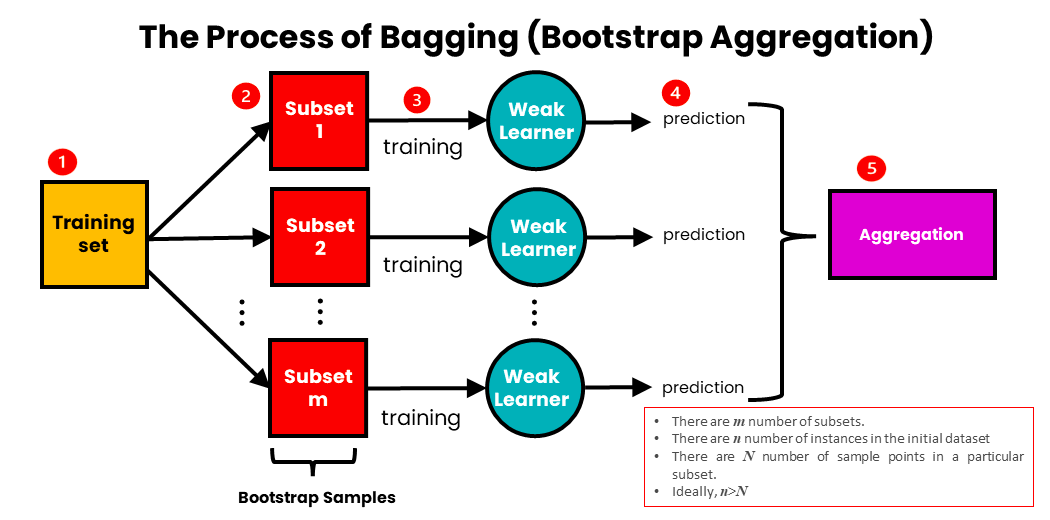
\includegraphics[width=0.85\textwidth]{chapitre1/figures/the proccess of Bagging.png}
  \caption{Schéma pédagogique du bagging : du jeu de données original aux échantillons bootstrap, puis aux modèles de base et à l'agrégation.}
  \label{fig:bagging-schema}
\end{figure}

\paragraph{Rôle des données out-of-bag (OOB).}
Lors de la génération de $D_i$, chaque exemple de $D$ a une probabilité $(1 - 1/n)^n \simeq 1/e$
de ne jamais être sélectionné ; environ $36{,}8\,\%$ des observations restent donc en dehors de
chaque bootstrap et sont dites \emph{out-of-bag} pour le modèle $\hat{f}_i$ considéré.

Pour une observation $(x_j, y_j)$, on note
\[
  S_j = \{\, i \in \{1,\dots,m\} \mid (x_j, y_j) \notin D_i \,\}
\]
l'ensemble des indices de modèles qui n'ont pas vu ce point à l'entraînement. On peut alors
d{\'e}finir une prédiction OOB par
\[
  \tilde{f}_j(x_j) = \frac{1}{|S_j|} \sum_{i \in S_j} \hat{f}_i(x_j)
\]
en régression, ou par vote majoritaire restreint aux $i \in S_j$ en classification. Une estimation
de l'erreur OOB est donnée par
\[
  \varepsilon_{\text{OOB}}
  = \frac{1}{n} \sum_{j=1}^n \ell\bigl(\tilde{f}_j(x_j), y_j\bigr),
\]
où $\ell$ est la fonction de perte (MSE, entropie croisée, etc.). Cette quantité fournit une
approximation fiable de l'erreur de généralisation, sans avoir besoin de réserver un jeu de
validation distinct~\cite{breiman_bagging_1996,eric_td4_ensemble,ibm_bagging}.

\paragraph{Réduction de la variance.}
Le principal intérêt du bagging est de réduire la variance des prédictions. Dans un scénario
idéal où les modèles $\hat{f}_i$ seraient indépendants et de variance $v$, la variance de la
moyenne
\[
  \hat{f}(x) = \frac{1}{m} \sum_{i=1}^m \hat{f}_i(x)
\]
serait $v/m$. En pratique, les modèles ne sont pas indépendants ; si l'on note $\rho$ la corrélation
moyenne entre deux prédicteurs, on obtient approximativement~\cite{cmu_ensembles_pdf} :
\[
  \operatorname{Var}\bigl[\hat{f}(x)\bigr]
  \approx \rho v + \frac{1 - \rho}{m}\,v.
\]
Quand $m$ augmente, le second terme décroît comme $1/m$ et la variance tend vers $\rho v$.
Le bagging est donc particulièrement pertinent lorsque les modèles de base sont peu biaisés
mais très variables (comme les arbres profonds) : il stabilise leurs prédictions sans augmenter
significativement le biais.

\paragraph{Exemples d'algorithmes baggés.}

\emph{Forêt aléatoire.}
La forêt aléatoire (\emph{Random Forest}) est l'extension la plus célèbre du bagging. En plus du
bootstrapping, elle introduit une randomisation des caractéristiques (\emph{features}) : à chaque
division d'un n\oe ud de l'arbre, seul un sous-ensemble aléatoire de variables est considéré.
Cela décorrèle les arbres et renforce encore la réduction de variance
~\cite{breiman_bagging_1996,ibm_bagging}.

Un aperçu schématique de l'algorithme Random Forest est donné par la
figure~\ref{fig:rf-overview}.

\begin{figure}[h]
  \centering
  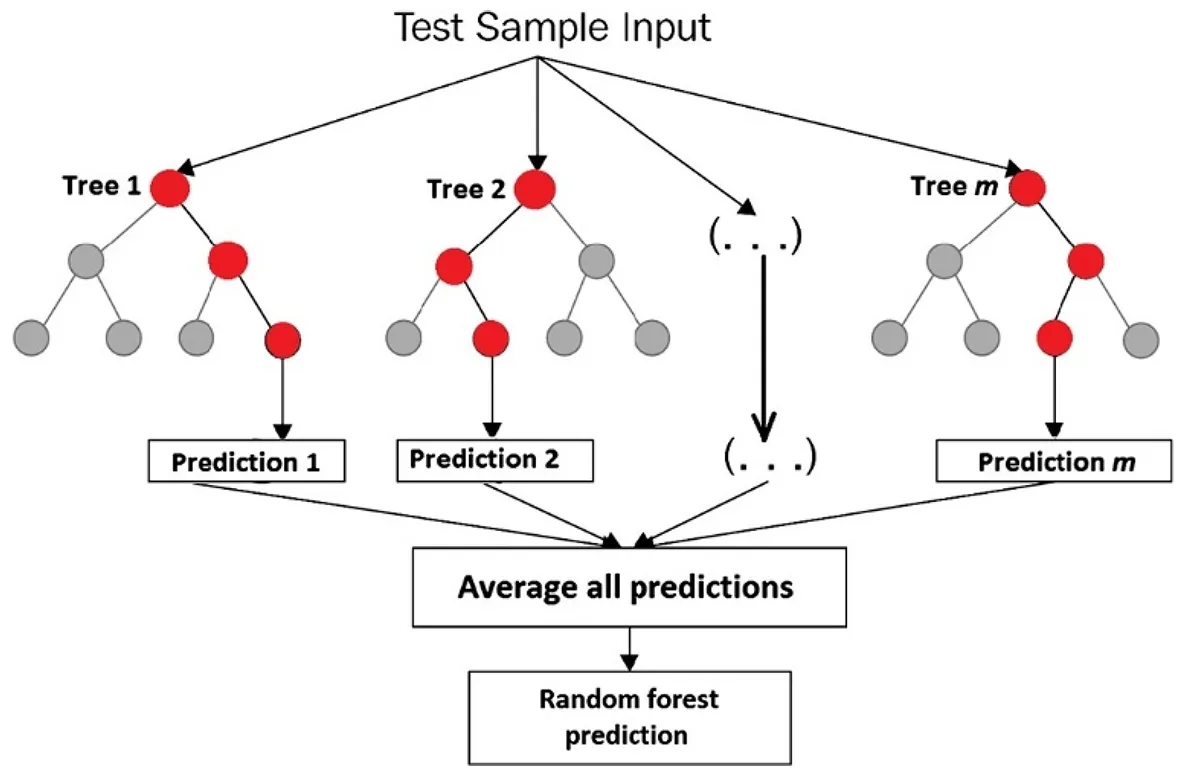
\includegraphics[width=0.7\textwidth]{chapitre1/figures/Aperçu de l'algorithme Random Forest(.png}
  \caption{Aperçu de l'algorithme Random Forest.}
  \label{fig:rf-overview}
\end{figure}

\paragraph{Exemple : bagging avec $k$ plus proches voisins.}
Le bagging ne se limite pas aux arbres. Par exemple, appliqué au classifieur des $k$ plus proches
voisins ($k$-NN), il permet de stabiliser un modèle naturellement très sensible aux fluctuations
locales des données. On génère $m$ jeux bootstrap $D_i$, chacun servant de base à un modèle
$k$-NN (qui consiste essentiellement à mémoriser $D_i$). Pour une nouvelle observation $x$, on
agrège les $m$ prédictions $k$-NN par vote ou moyenne des probabilités estimées
~\cite{gfg_ensemble_learning,mlm_bagging_vs_boosting_vs_stacking}.

Dans les bibliothèques modernes comme scikit-learn, ces variantes sont disponibles via la
classe \texttt{BaggingClassifier} en choisissant simplement l'estimateur de base (arbre,
$k$-NN, etc.) et en activant le calcul de la \og OOB score \fg{} pour obtenir automatiquement
une estimation interne de l'erreur de généralisation.

\subsection{Boosting}

Le boosting regroupe une famille de méthodes séquentielles où les modèles sont entraînés les
uns après les autres, chacun se concentrant sur les erreurs commises par les précédents. Contrairement
au bagging qui agit surtout sur la variance, le boosting cherche principalement à
réduire le biais, en construisant progressivement un modèle additif puissant à partir de
modèles de base faibles~\cite{freund_schapire_adaboost_1997,schapire_boosting_intro_1999,mlm_bagging_vs_boosting_vs_stacking,greatlearning_bagging_boosting}.

\paragraph{Principe général.}
On considère un ensemble d'entraînement $\{(x_i, y_i)\}_{i=1}^n$ avec $y_i \in \{-1, +1\}$ pour
fixer les idées. Le boosting maintient une distribution de poids $D_t(i)$ sur les exemples. À
chaque itération $t$ :
\begin{enumerate}
  \item un \emph{apprenant faible} $h_t$ est entraîné sur les données pondérées par $D_t$ ;
  \item son erreur pondérée $\varepsilon_t = \sum_i D_t(i)\,\mathbb{I}\bigl(h_t(x_i) \neq y_i\bigr)$ est évaluée ;
  \item un coefficient $\alpha_t$ mesurant la confiance accordée à $h_t$ est calculé ;
  \item les poids $D_t$ sont mis à jour pour donner plus d'importance aux exemples mal
  prédits.
\end{enumerate}
Le modèle final est une combinaison pondérée des $h_t$. Sous l'hypothèse de \og faible
apprentissage \fg{} (chaque $h_t$ fait un peu mieux que le hasard), on peut montrer que l'erreur
d'entraînement décroît de manière exponentielle avec le nombre d'itérations
~\cite{freund_schapire_adaboost_1997,schapire_boosting_intro_1999}.

\begin{figure}[h]
  \centering
  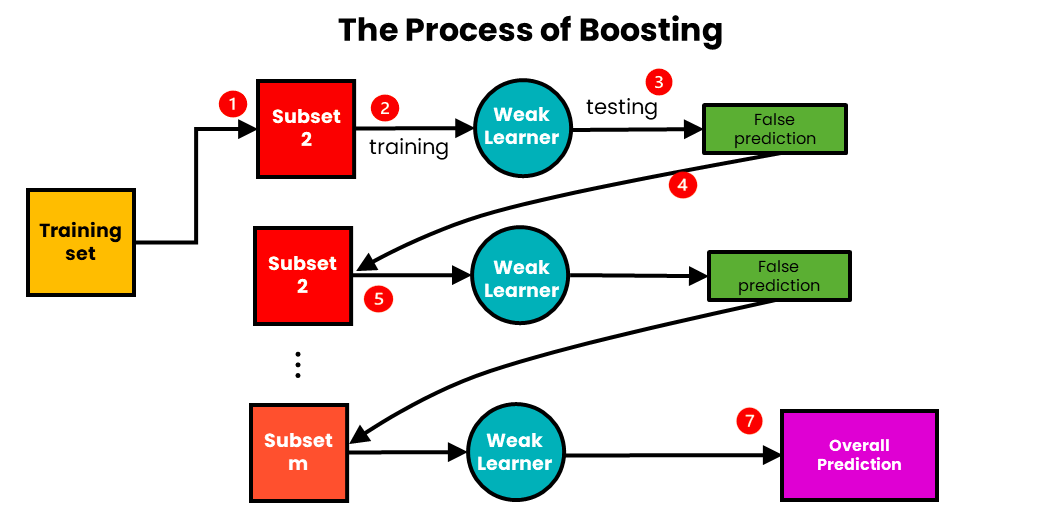
\includegraphics[width=0.85\textwidth]{chapitre1/figures/the_process_of_boosting.png}
  \caption{Schéma pédagogique du boosting : chaîne de modèles où chaque étape corrige les erreurs de la précédente.}
  \label{fig:boosting-schema}
\end{figure}

\paragraph{AdaBoost : formulation et réduction du biais.}
AdaBoost (Adaptive Boosting) est l'algorithme de boosting le plus classique
~\cite{freund_schapire_adaboost_1997,schapire_boosting_intro_1999}. Sa version binaire peut
se décrire comme suit.

\begin{enumerate}
  \item \textbf{Initialisation.} On part d'une distribution uniforme
  \[
    D_1(i) = \frac{1}{n}, \quad i = 1,\dots,n.
  \]

  \item \textbf{Pour $t = 1,\dots,T$ :}
  \begin{enumerate}
    \item on entraîne un modèle faible $h_t : \mathcal{X} \to \{-1,+1\}$ en minimisant l'erreur
    pondérée
    \[
      \varepsilon_t = \sum_{i=1}^n D_t(i)\,\mathbb{I}\bigl(h_t(x_i) \neq y_i\bigr),
    \]
    avec la contrainte $\varepsilon_t < 1/2$ ;

    \item on définit le poids du modèle
    \[
      \alpha_t = \frac{1}{2}\,\log\!\left(\frac{1 - \varepsilon_t}{\varepsilon_t}\right) ;
    \]

    \item on met à jour les poids des exemples :
    \[
      D_{t+1}(i)
      = \frac{D_t(i)\,\exp\bigl(-\alpha_t y_i h_t(x_i)\bigr)}{Z_t},
    \]
    où $Z_t$ est un facteur de normalisation assurant $\sum_i D_{t+1}(i) = 1$. Les exemples
    mal classés ($y_i h_t(x_i) < 0$) voient leur poids augmenter, ce qui force $h_{t+1}$ à se
    focaliser sur eux.
  \end{enumerate}
\end{enumerate}

Le classifieur final est
\[
  H(x) = \operatorname{sign}\!\left(\sum_{t=1}^T \alpha_t h_t(x)\right).
\]
Théoriquement, on peut montrer que l'erreur d'entraînement de $H$ est majorée par
~\cite{schapire_boosting_intro_1999,freund_schapire_adaboost_1997}
\[
  \mathrm{err}_{\text{train}}(H)
  \leq \prod_{t=1}^T Z_t
  \leq \exp\!\left(-2\sum_{t=1}^T \gamma_t^2\right),
  \quad
  \text{où } \gamma_t = \tfrac{1}{2} - \varepsilon_t.
\]
Si chaque apprenant faible est au moins un peu meilleur que le hasard ($\gamma_t \ge \gamma > 0$),
l'erreur d'entraînement décroît donc comme $\exp(-2\gamma^2 T)$. En pratique, cela signifie
que le biais du modèle global diminue rapidement avec le nombre d'itérations, tant que les
apprenants restent effectivement faibles et diversifiés.

On peut aussi interpréter AdaBoost comme une méthode qui minimise de façon gloutonne la
perte exponentielle
\[
  L(f) = \sum_{i=1}^n \exp\!\bigl(-y_i f(x_i)\bigr),
  \quad f(x) = \sum_{t=1}^T \alpha_t h_t(x),
\]
par une descente de gradient coordonnée dans l'espace des fonctions. Cette vision explique
pourquoi la marge $y_i f(x_i)$ joue un rôle central dans la performance~\cite{schapire_boosting_intro_1999}.

En pratique, AdaBoost est souvent implémenté avec des \emph{decision stumps} (arbres de
profondeur 1) comme apprenants faibles ; dans scikit-learn, on peut l'utiliser via la classe
\texttt{AdaBoostClassifier} avec un \texttt{DecisionTreeClassifier(max\_depth=1)} comme estimateur
de base. La complexité est en gros proportionnelle à $T$ fois le coût d'entraînement d'un
apprenant faible, et l'algorithme est naturellement itératif.

\paragraph{Gradient boosting : point de vue en espace de fonctions.}
Le gradient boosting généralise l'idée du boosting à toute fonction de perte différentiable
~\cite{friedman_gbm_2001}. On cherche à approximer une fonction $F^\star$ en construisant un
modèle additif
\[
  F_T(x) = \sum_{t=1}^T \nu\,\beta_t\,h_t(x),
\]
où $h_t$ sont des apprenants faibles (souvent des arbres de décision), $\beta_t$ des coefficients
et $\nu \in (0,1]$ un facteur de \og shrinkage \fg{} (taux d'apprentissage).

À chaque itération $t$ :
\begin{enumerate}
  \item on dispose d'un modèle courant $F_{t-1}$ ;
  \item on calcule, pour chaque exemple, les \emph{pseudo-résidus} correspondant au gradient
  négatif de la perte par rapport aux prédictions :
  \[
    r_{it}
    = -\left.\frac{\partial}{\partial F(x_i)} L\bigl(y_i, F(x_i)\bigr)\right|_{F = F_{t-1}};
  \]
  pour une perte quadratique, on obtient simplement $r_{it} = y_i - F_{t-1}(x_i)$ ;

  \item on ajuste un apprenant faible $h_t$ pour approximer ces pseudo-résidus, typiquement par
  régression aux moindres carrés :
  \[
    h_t \approx \arg\min_h \sum_{i=1}^n \bigl(r_{it} - h(x_i)\bigr)^2 ;
  \]

  \item on choisit un pas optimal $\beta_t$ (par recherche de ligne) :
  \[
    \beta_t = \arg\min_{\beta} \sum_{i=1}^n
      L\bigl(y_i, F_{t-1}(x_i) + \beta\,h_t(x_i)\bigr),
  \]
  puis on met à jour
  \[
    F_t(x) = F_{t-1}(x) + \nu\,\beta_t\,h_t(x).
  \]
\end{enumerate}

Pour la régression (perte quadratique), cela revient à ajuster successivement les résidus
$y_i - F_{t-1}(x_i)$ ; pour la classification logistique, les pseudo-résidus correspondent à une
erreur sur les probabilités estimées. Ainsi, chaque itération corrige systématiquement l'erreur
résiduelle, ce qui diminue le biais tout en permettant un contrôle fin de la complexité via
$\nu$, la profondeur des arbres et le nombre d'itérations~\cite{friedman_gbm_2001}.

Des implémentations standards existent dans scikit-learn (\texttt{GradientBoostingClassifier},
\texttt{GradientBoostingRegressor}) ainsi que dans des bibliothèques dédiées comme XGBoost et
LightGBM.

\paragraph{XGBoost et LightGBM : optimisations modernes.}
XGBoost~\cite{chen_guestrin_xgboost_2016} et LightGBM~\cite{ke_lightgbm_2017} sont des
implémentations très optimisées du gradient boosting sur arbres de décision, qui ajoutent
plusieurs idées clés :
\begin{itemize}
  \item utilisation d'un développement de Taylor d'ordre 2 de la perte pour calculer, pour chaque
  feuille candidate, le gain associé à une scission en fonction de la somme des gradients
  $G$ et des hessiennes $H$ ;

  \item régularisation explicite des arbres via des termes de pénalisation $L_2$ sur les poids des
  feuilles et une pénalité sur le nombre de feuilles (paramètres $\lambda$ et $\gamma$) ;

  \item sous-échantillonnage des observations et des variables (\emph{row/column subsampling})
  pour réduire la corrélation entre arbres et accélérer l'entraînement ;

  \item structures de données basées sur des histogrammes et croissance feuille-par-feuille
  (LightGBM) pour optimiser l'utilisation de la mémoire et du CPU.
\end{itemize}

Par exemple, dans XGBoost, le gain d'une scission est approximativement donné par
~\cite{chen_guestrin_xgboost_2016}
\[
  \operatorname{Gain}
  = \frac{1}{2}
    \left(
      \frac{G_L^2}{H_L + \lambda}
      + \frac{G_R^2}{H_R + \lambda}
      - \frac{(G_L + G_R)^2}{H_L + H_R + \lambda}
    \right)
    - \gamma,
\]
où $G_L, H_L$ (resp. $G_R, H_R$) sont les sommes des gradients et hessiennes dans les feuilles
gauche et droite. Cette expression permet de choisir efficacement les meilleures scissions.

Du point de vue pratique, XGBoost et LightGBM sont devenus des standards de facto pour les
problèmes tabulaires de grande dimension, grâce à leur excellent compromis entre biais (faible)
et variance contrôlée par une régularisation riche et de nombreux hyperparamètres.



\subsection{Stacking (stacked generalization)}

Le stacking, ou \emph{stacked generalization}, est une méthode d'ensemble à deux niveaux où un
modèle dit \emph{méta-modèle} apprend comment combiner au mieux les prédictions de plusieurs
modèles de base~\cite{wolpert_stacked_1992,ting_witten_stacking_1999}. Contrairement au vote
ou à la simple moyenne, les poids de combinaison sont appris à partir des données, ce qui permet
souvent de réduire l'erreur quadratique moyenne (MSE) en régression, ou l'erreur de classification,
par rapport à chaque modèle pris isolément~\cite{breiman_stacked_regressions_1996}.

\paragraph{Architecture en couches.}
On distingue classiquement deux niveaux~\cite{wolpert_stacked_1992,ting_witten_stacking_1999} :
\begin{itemize}
  \item \textbf{Niveau 0 (apprenants de base)} : plusieurs modèles potentiellement très différents
  (forêt aléatoire, gradient boosting, SVM, k-NN, réseaux neuronaux, etc.) sont entraînés sur
  les données d'entrée $x$ pour prédire $y$ ;

  \item \textbf{Niveau 1 (méta-modèle)} : un dernier modèle (souvent une régression linéaire pour la
  régression, ou une régression logistique pour la classification) prend en entrée les
  prédictions des modèles de niveau 0 et apprend une combinaison optimale.
\end{itemize}

En notation matricielle pour un problème de régression, si l'on dispose de $K$ modèles de
base produisant des prédictions $\hat{y}_k^{(i)}$ pour l'observation $i$, on forme la matrice de
caractéristiques de niveau 1 :
\[
  Z =
  \begin{bmatrix}
    \hat{y}_1^{(1)} & \dots & \hat{y}_K^{(1)} \\
    \vdots          &       & \vdots          \\
    \hat{y}_1^{(n)} & \dots & \hat{y}_K^{(n)}
  \end{bmatrix},
  \quad
  y =
  \begin{bmatrix}
    y^{(1)} \\
    \vdots  \\
    y^{(n)}
  \end{bmatrix}.
\]
Le méta-modèle linéaire cherche alors des coefficients $w \in \mathbb{R}^K$ tels que
\[
  \hat{y}^{\text{stack}} = Z w
\]
approche au mieux $y$ au sens de la MSE. Le choix de $w$ se fait en minimisant
\[
  \min_w \|y - Z w\|_2^2,
\]
éventuellement sous la contrainte $w_k \ge 0$ comme proposé par Breiman
~\cite{breiman_stacked_regressions_1996}. Cette contrainte de non-négativité aide à garantir
que le stacking ne dégrade pas les performances par rapport aux meilleurs modèles de base.

\begin{figure}[h]
  \centering
  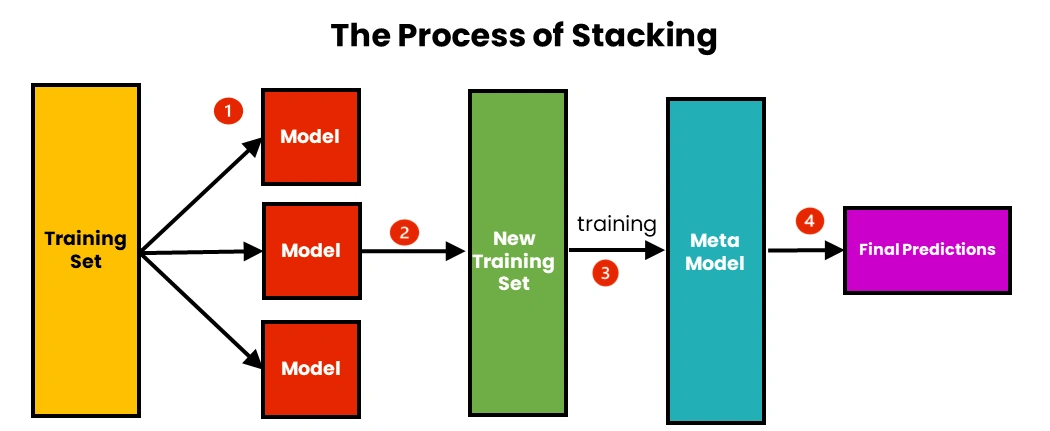
\includegraphics[width=0.8\textwidth]{chapitre1/figures/the process of stacking.png}
  \caption{Schéma pédagogique du stacking : architecture en couches avec apprenants de niveau 0 et méta-modèle de niveau 1.}
  \label{fig:stacking-schema}
\end{figure}

\paragraph{Le problème du \og data leakage \fg{}.}
Une implémentation naïve du stacking consisterait à entraîner les modèles de base sur tout
le jeu d'entraînement $D_{\text{train}}$ et à utiliser leurs prédictions sur ces mêmes exemples
comme méta-caractéristiques :
\[
  Z_{ij}^{\text{na\"if}} = L_i(x_j),
  \quad (x_j,y_j) \in D_{\text{train}},
\]
où $L_i$ désigne le $i$-ème modèle de base. Dans ce cas, le méta-modèle est ajusté sur des
prédictions issues de données déjà vues par les modèles de niveau 0. On introduit ainsi une
fuite d'information (\emph{data leakage}) : les performances apparentes sur l'entraînement sont
très optimistes, et le méta-modèle apprend à exploiter des corrélations artificiellement fortes
entre les sorties des modèles de base et la cible~\cite{ting_witten_stacking_1999}.

Pour obtenir une estimation non biaisée des sorties des modèles de base, il faut s'assurer que,
pour chaque exemple $(x_j,y_j)$, les prédictions utilisées au niveau 1 proviennent de modèles
qui n'ont pas été entraînés sur $(x_j,y_j)$. La solution est d'utiliser des prédictions
\emph{out-of-fold} (OOF) construites par validation croisée interne.



\paragraph{Etapes algorithmiques (stacking avec validation croisée).}
La procédure standard de stacking avec prédictions OOF se déroule comme suit :
\begin{enumerate}
  \item \textbf{Sélection des modèles de base.} Le choix des apprenants de niveau 0 est crucial. On
  recherche :
  \begin{itemize}
    \item \textbf{Diversité} : des modèles capturant des aspects différents du problème (modèles
    linéaires, arbres, réseaux de neurones, SVM, $k$-NN, etc.) ;
    \item \textbf{Complémentarité} : des erreurs faiblement corrélées entre modèles, de sorte que
    chacun corrige les faiblesses des autres ;
    \item \textbf{Qualité individuelle} : chaque modèle doit être raisonnablement performant pris
    isolément (un modèle très mauvais reste difficile à rattraper par le stacking) ;
    \item \textbf{Hétérogénéité} : on privilégie des familles algorithmiques différentes plutôt que
    de nombreuses variantes très proches d'un même modèle.
  \end{itemize}

  \item \textbf{Découpage du jeu d'entraînement.} On partitionne le jeu de données en $K$ plis de
  validation croisée $F_1,\dots,F_K$.

  \item \textbf{Entraînement des modèles de base et génération des méta-caractéristiques.}
  Pour chaque pli $F_k$ :
  \begin{enumerate}
    \item on entraîne chaque modèle de base sur $D \setminus F_k$ ;
    \item on applique ces modèles à $F_k$ pour produire des prédictions $\hat{y}_k^{(i)}$ pour les
    exemples $i \in F_k$.
  \end{enumerate}
  En concaténant les prédictions sur tous les plis, on obtient, pour chaque exemple $i$, un
  vecteur $(\hat{y}_1^{(i)},\dots,\hat{y}_K^{(i)})$ obtenu sur des données \emph{out-of-fold}.

  \item \textbf{Apprentissage du méta-modèle.} On ajuste ensuite le méta-modèle sur la matrice
  $Z$ et les vraies cibles $y$. Le choix du méta-modèle dépend du type de tâche et du
  compromis biais/variance recherché. Quelques options courantes sont :
  \begin{itemize}
    \item \textbf{Régression linéaire / Ridge} : interprétable, stable, rapide ; bon choix par défaut
    en régression pour un premier essai ;
    \item \textbf{Régression logistique} : produit des probabilités bien calibrées ; adaptée à la
    classification binaire ;
    \item \textbf{Arbre de décision (profondeur modérée)} : permet de capturer des interactions
    non linéaires entre les sorties des modèles de base ;
    \item \textbf{Gradient boosting peu profond} : très performant lorsque l'on dispose de beaucoup
    de données et que l'on souhaite modéliser des combinaisons complexes de prédicteurs de
    niveau 0 ;
    \item \textbf{Réseau de neurones peu profond} : utile pour des schémas de stacking plus
    profonds ou lorsque les relations entre modèles de base sont fortement non linéaires.
  \end{itemize}
  En pratique, on privilégie souvent des méta-modèles simples (régression linéaire ou logistique)
  pour limiter le risque de surajustement au niveau 1.

  \item \textbf{Apprentissage final des modèles de base.} On réentraîne enfin tous les modèles de
  base sur la totalité du jeu d'entraînement, avant de les utiliser en test. En production, la
  prédiction d'un nouvel exemple $x^\star$ se fait en deux temps : (i) chaque modèle de base
  produit une prédiction ; (ii) le méta-modèle agrège ces prédictions.
\end{enumerate}

Cette procédure garantit que le méta-modèle a vu des prédictions réalistes (obtenues sur des
échantillons non vus par les modèles de base), évitant ainsi un surajustement massif.

\paragraph{Reduction du Biais et la Variance }
Le stacking agit à deux niveaux :
\begin{itemize}
  \item \textbf{Réduction du biais}le méta-learner apprend à corriger les erreurs systématiques des base learners en apprenant une combinaison non-linéaire (si le méta est un arbre ou un réseau).
  \item \textbf{Réduction de la variance} en utilisant des prédictions croisées, il évite le surajustement et agit comme un régulariseur ; la variance finale est souvent inférieure à celle d’un simple vote ou moyenne.
\end{itemize}
Mathématiquement, si les erreurs des apprenants de base sont peu corrélées, la variance de la prédiction combinée est proche de
\[
  \text{Var}\left(\sum_{i=1}^K w_i h_i(x)\right) \approx \sum_{i=1}^K w_i^2\,\text{Var}(h_i(x)),
\]
où $h_i$ désigne un modèle de base et $w_i$ les poids appris par le méta-modèle. Dans le cas d'un simple stacking avec moyenne ($w_i = 1/K$), on retrouve
\[
  \text{Var}_{\text{ensemble}} \approx \frac{1}{K} \sum_{i=1}^K \text{Var}\bigl(h_i(x)\bigr)
\]



\paragraph{Limites et risques du stacking.}
Malgré ses qualités, le stacking présente plusieurs limites qu'il faut garder à l'esprit :
\begin{itemize}
  \item \textbf{Surapprentissage du méta-modèle} : si les lignes de $Z$ sont trop corrélées à $y$
  (par exemple en cas de mauvais schéma OOF), le méta-modèle peut mémoriser des
  patterns propres au jeu d'entraînement plutôt que des relations généralisables.
  \item \textbf{Coût computationnel} : la génération des prédictions OOF nécessite d'entraîner chaque
  modèle de base sur plusieurs plis (environ $K \times F$ entraînements), puis d'entraîner le
  méta-modèle ; cela peut devenir coûteux pour de grands ensembles ou des modèles lourds.
  \item \textbf{Complexité de déploiement} : en production, il faut maintenir $K$ modèles de base
  plus le méta-modèle, ce qui complique la mise à jour, la surveillance et l'observabilité.
  \item \textbf{Interprétabilité réduite} : le système forme une boîte noire à deux niveaux ; il est
  souvent difficile d'expliquer précisément pourquoi une décision a été prise.
  \item \textbf{Risque de leakage} : toute fuite d'information dans la génération des prédictions OOF
  (par exemple partage involontaire de données entre plis) invalide les hypothèses
  théoriques et peut conduire à un méta-modèle fortement biaisé.
\end{itemize}

\subsection{Voting (vote majoritaire vs vote probabiliste)}

Le vote est la méthode de fusion la plus simple pour les modèles parallèles~\cite{codefinity_voting,gfg_voting_classifier}.

\paragraph{Hard voting (vote majoritaire).}

Chaque modèle donne une étiquette de classe. On choisit la classe qui a reçu le plus de
suffrages. Par exemple :

\begin{itemize}
  \item Modèle A $\rightarrow$ \og chien \fg{}
  \item Modèle B $\rightarrow$ \og chat \fg{}
  \item Modèle C $\rightarrow$ \og chien \fg{}
\end{itemize}

La décision finale est alors \og chien \fg{} (deux voix contre une).

\paragraph{Soft voting (vote probabiliste).}

On calcule la moyenne des probabilités prédites pour chaque classe. Cette méthode est plus
précise car elle accorde plus d'importance aux modèles \og sûrs d'eux \fg{}.

Considérons par exemple deux classes (chat, chien) et trois modèles :
\begin{itemize}
  \item Modèle 1 : probabilités $[P(\text{chien}) = 0{,}4,\; P(\text{chat}) = 0{,}6]$ $\Rightarrow$ prédit \og chat \fg{}
  \item Modèle 2 : probabilités $[0{,}4,\; 0{,}6]$ $\Rightarrow$ prédit \og chat \fg{}
  \item Modèle 3 : probabilités $[0{,}9,\; 0{,}1]$ $\Rightarrow$ prédit \og chien \fg{}
\end{itemize}

En hard voting, la classe \og chat \fg{} (deux voix) l'emporte. En soft voting, on calcule :
\[
  \overline{P}(\text{chien}) = \frac{0{,}4 + 0{,}4 + 0{,}9}{3} \approx 0{,}56,\qquad
  \overline{P}(\text{chat})  = \frac{0{,}6 + 0{,}6 + 0{,}1}{3} \approx 0{,}43.
\]
La décision finale est alors \og chien \fg{} : la forte conviction du modèle 3 compense l'incertitude
des deux autres.

\section{Analyse comparative des approches}

Le choix d'une méthode d'ensemble dépend des contraintes du projet (volume de données,
temps de réponse, précision requise, robustesse au bruit, coût de calcul, etc.).

Le tableau suivant résume quelques caractéristiques essentielles des trois grandes familles :

\begin{table}[h]
  \centering
  \caption{Comparaison synthétique bagging / boosting / stacking}
  \begin{tabular}{llll}
    \toprule
    Critère & Bagging & Boosting & Stacking \\
    \midrule
    Objectif principal
      & Réduire la variance
      & Réduire le biais
      & Maximiser la précision \\
    Type de modèles
      & Homogènes (arbres profonds)
      & Homogènes (arbres peu profonds)
      & Hétérogènes (divers types) \\
    Entraînement
      & Parallèle (indépendant)
      & Séquentiel (dépendant)
      & Parallèle + méta-apprentissage \\
    Sensibilité au bruit
      & Faible (robuste)
      & Élevée (risque de sur-ajuster)
      & Variable \\
    Risque d'overfitting
      & Faible
      & Élevé (si non régularisé)
      & Moyen (si données limitées) \\
    Coût de calcul
      & Efficace (parallélisable)
      & Lent (entraînement en série)
      & Très élevé \\
    \bottomrule
  \end{tabular}
\end{table}


\section{Avantages et limites de la combinaison}

\subsection{Avantages}

\begin{enumerate}
  \item \textbf{Précision supérieure} : les ensembles dépassent quasi systématiquement les modèles
  uniques en combinant des perspectives complémentaires.

  \item \textbf{Généralisation et robustesse} : en lissant les prédictions, les systèmes MCS sont moins
  sensibles aux anomalies statistiques d'un seul jeu de données.

  \item \textbf{Traitement des données complexes} : ils permettent de diviser un problème complexe
  en sous-tâches traitées par des experts dédiés (\emph{divide and conquer}).
\end{enumerate}

\subsection{Limites}

\begin{enumerate}
  \item \textbf{Coût en ressources} : l'entraînement de dizaines ou de centaines de modèles consomme
  du temps CPU, de la mémoire et de l'énergie.

  \item \textbf{Opacité (\og black box \fg{})} : il est extrêmement difficile d'expliquer pourquoi un ensemble de
  plusieurs centaines d'arbres de décision a pris une décision spécifique.

  \item \textbf{Complexité de maintenance} : gérer un pipeline avec plusieurs modèles hétérogènes
  demande une infrastructure plus lourde qu'un modèle monolithique.
\end{enumerate}

\section*{Conclusion}

La combinaison de classifieurs représente une approche mature et extrêmement puissante de
l'apprentissage automatique. En orchestrant judicieusement la diversité et en s'appuyant sur
des fondements statistiques rigoureux, les systèmes multi-classifieurs permettent de
transformer une collection de modèles imparfaits en un outil de décision d'une fiabilité
exceptionnelle~\cite{ibm_ensemble_learning,ultralytics_ensemble_role,gfg_ensemble_learning,luisfredgs_mcs_intro}.

